%\section{Une section}

% remarque : pour qu'un mot se retrouve dans le lexique : \MotDefinition{asymptote horizontale}{} 

\begin{methode*1}[Construire le symétrique d'un point à l'équerre]

\begin{aconnaitre}
Le \MotDefinition{symétrique d'un point $P$}{} par rapport à une droite $d$ est le point $S$ tel que la droite $d$ soit la médiatrice du segment $[PS]$. 
\end{aconnaitre}

\begin{exemple*1}
Construis le point $S$, symétrique de $P$ par rapport à la droite $d$, en utilisant l'équerre : \\[.5em]

\begin{tabularx}{\textwidth}{X|X|X}
 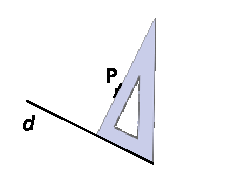
\includegraphics[width=2.4cm]{equerredP} &  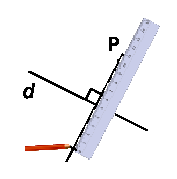
\includegraphics[width=2.4cm]{equerredP_perp} & 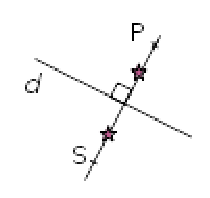
\includegraphics[width=2.2cm]{SymP} \\ 
 On construit la droite perpendiculaire à la droite $d$ passant par le point $P$. & On reporte la distance de $P$ à $(d)$ de l'autre côté de $d$ sur cette perpendiculaire. & On obtient ainsi le point $S$ tel que $d$ soit la médiatrice de $[PS]$. \\
\end{tabularx} \\

%\begin{tabularx}{\textwidth}{X|X|X}
% 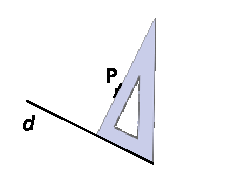
\includegraphics[width=2.4cm]{equerredP} &  %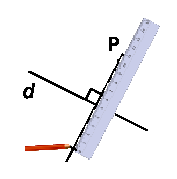
\includegraphics[width=2.4cm]{equerredP_perp} & %\includegraphics[width=2.2cm]{symP} \\ 
% On construit la droite perpendiculaire à la droite $d$ passant par le point $P$. & On reporte la distance de $P$ à $(d)$ de l'autre côté de $d$ sur cette perpendiculaire. & On obtient ainsi le point $S$ tel que $d$ soit la médiatrice de $[PS]$.\\
%\end{tabularx}\\
 \end{exemple*1}


\exercice
Trace deux droites sécantes $d'$ et $d''$ puis place un point $A$ qui n'appartient ni à $d'$, ni à $d''$. Construis les symétriques $A'$ et $A''$ de $A$ par rapport à $d'$ et à $d''$.
%\correction
 
\end{methode*1}

%%%%%%%%%%%%%%%%%%%%%%%%%%%%%%%%%%%%%%%%%%%%%%%%%%%%%%%%%%%%%%%%%%%%%

\begin{methode*1}[Construire le symétrique d'un point au compas]

\begin{aconnaitre}
Si $A$ et $B$ sont symétriques par rapport à une droite $d$ alors chaque point de la droite $d$ est \MotDefinition{équidistant}{} de $A$ et de $B$. 
\end{aconnaitre}

\begin{exemple*1}
Construis le point $S$, symétrique de $P$ par rapport à la droite $d$, au compas seul : \\[0.5em]
\begin{tabularx}{\textwidth}{X|X|X}
 
\newcommand{\NodeAngle}[2]{%
    %\pgfextra{
        \pgfmathanglebetweenpoints%
            {\pgfpointanchor{#1}{center}}%
            {\pgfpointanchor{#2}{center}}%
            \global\let\MyAngle\pgfmathresult
    }%}

    % #1 premier point              ---- Distance entre 2 nodes ----
    % #2 second point
    % On récupère le résultat dans \MyDist
\makeatletter
\newcommand{\NodeDist}[2]{%
    \pgfpointdiff{\pgfpointanchor{#1}{center}}
                 {\pgfpointanchor{#2}{center}}
    % no need to use a new dimen
    \pgf@xa=\pgf@x
    \pgf@ya=\pgf@y
    % to convert from pt to cm   
    \pgfmathparse{veclen(\pgf@xa,\pgf@ya)/28.45274}
    \global\let\MyDist\pgfmathresult % we need a global macro   
}
\makeatother

% ######################
%     Dessin crayon    #
% ######################

\newcommand{\Crayon}[1]{%
    \begin{scope}[scale=.7,#1]
    \fill[gray!60] (-.2,4.8) -- (.2,4.8)
                -- (.2,.8) --(.1,.65)
                -- (0,.8) -- (-.1,.66)
                -- (-.2,.8) -- cycle ;
    \draw[color=white] (0,4.8) -- (0,.8 );
    \fill[black] (-.2,4.3) -- (0,4.27)
                -- (.2,4.3) -- (.2,4.8) arc(30:150:0.23cm) ;
    \fill[brown!50] (-.2,.8)
        -- (0,0) node[coordinate,pos=0.75](a){}
        -- (.2,.8) node[coordinate,pos=0.25](b){}
        -- (.1,.65) -- (0,.8) -- (-.1,.66) -- cycle;
    \fill[gray] (a) -- (0,0) -- (b) -- cycle;
    \end{scope}
}



% ######################
%   Dessin du compas   #
% ######################

\NewDocumentCommand{\Compas}{smm}{%

    \IfBooleanTF{#1}{%
    % with *
    % keep distance between extemities
    }{%
    % without *
    % calulation of the distance between extemities
    \NodeDist{#2}{#3}
    }

    \NodeAngle{#2}{#3}

    \def\L{6} % taille des branches du compas

    % calcul de l'angle de l'ouverture
    \pgfmathsetmacro{\AngleCP}{asin(\MyDist/(2*\L))}

    \begin{scope}[shift=(#2)]
    \begin{scope}[%
        join=round,
        rotate=\MyAngle,
        shift=(270-\AngleCP:-\L)
        ]

    % branche pointe sèche
    \draw[rotate=-\AngleCP,fill=gray!80]
        (0,0)--(0,-\L)--(-.2,-\L+.8)--(-.2,0)--cycle ;
    \draw[rotate=-\AngleCP,fill=gray!05]
        (0,-\L+.8)--(0,-\L)--(-.2,-\L+.8)--cycle ;

    % branche crayon
    \draw[rotate=\AngleCP,fill=gray!80]
        (0,0)--(0,-\L)--(.2,-\L+.8)--(.2,0)--cycle ;

    \begin{scope}[rotate=\AngleCP,shift={(0,-\L)}]
    \Crayon{rotate=-12}
    \draw[fill=gray!25] (\L/30,\L/5) circle (\L/36) ;
    \fill[gray!5] (\L/30,\L/5)
            -- ++(30:\L/36) arc (30:45:\L/36) -- cycle ;
    \fill[gray!5] (\L/30,\L/5)
            -- ++(210:\L/36) arc (210:225:\L/36) ;
    \filldraw (\L/30,\L/5) circle (.02) ;
    \end{scope}

    % haut du compas
    \draw[fill=gray!80] (-.1,0) rectangle (.1,.7) ;
    \draw[fill=gray!25] (0,0) circle (.25) ;
    \fill[gray!5] (0,0) -- (30:.25) arc (30:45:.25) -- cycle ;
    \fill[gray!5,rotate=180] (0,0) -- (30:.25) arc (30:45:.25) -- cycle ;
    \filldraw (0,0) circle (.05) ;
    \end{scope}
    \end{scope}
}





\scalebox{.2}{
\begin{tikzpicture}	
  
    
\def \CharSize {3};
\def \BulletSize {2};

\coordinate (A) at (0,0) ;
\coordinate (P) at (2,4) ;
\coordinate (M) at (-4,2) ;
\coordinate (N) at (4,-2) ;

\Compas{P}{M}

%droite d
\draw[very thick] (-8,4)--(8,-4);
\draw (-6,4) node [scale=\CharSize]{$d$};

%point P
\draw (P) node [above,scale=\CharSize]{P};
\draw (P) node[scale=\BulletSize]{$\times$};

%arcs de cercle marqués par le compas
\draw [thick, color=gray](-4,2) arc(198.4:185:6.32);
\draw [thick, color=gray](-4,2) arc(198.4:211.8:6.32);
\draw [thick, color=gray](4,-2) arc(-71.6:-58.6:6.32);
\draw [thick, color=gray](4,-2) arc(-71.6:-84.6:6.32);
%\draw [color=red](P) circle (6.32);

\end{tikzpicture} 
 } %fin de la scalebox
 &
 
\newcommand{\NodeAngle}[2]{%
    %\pgfextra{
        \pgfmathanglebetweenpoints%
            {\pgfpointanchor{#1}{center}}%
            {\pgfpointanchor{#2}{center}}%
            \global\let\MyAngle\pgfmathresult
    }%}

    % #1 premier point              ---- Distance entre 2 nodes ----
    % #2 second point
    % On récupère le résultat dans \MyDist
\makeatletter
\newcommand{\NodeDist}[2]{%
    \pgfpointdiff{\pgfpointanchor{#1}{center}}
                 {\pgfpointanchor{#2}{center}}
    % no need to use a new dimen
    \pgf@xa=\pgf@x
    \pgf@ya=\pgf@y
    % to convert from pt to cm   
    \pgfmathparse{veclen(\pgf@xa,\pgf@ya)/28.45274}
    \global\let\MyDist\pgfmathresult % we need a global macro   
}
\makeatother

% ######################
%     Dessin crayon    #
% ######################

\newcommand{\Crayon}[1]{%
    \begin{scope}[scale=.7,#1]
    \fill[gray!60] (-.2,4.8) -- (.2,4.8)
                -- (.2,.8) --(.1,.65)
                -- (0,.8) -- (-.1,.66)
                -- (-.2,.8) -- cycle ;
    \draw[color=white] (0,4.8) -- (0,.8 );
    \fill[black] (-.2,4.3) -- (0,4.27)
                -- (.2,4.3) -- (.2,4.8) arc(30:150:0.23cm) ;
    \fill[brown!50] (-.2,.8)
        -- (0,0) node[coordinate,pos=0.75](a){}
        -- (.2,.8) node[coordinate,pos=0.25](b){}
        -- (.1,.65) -- (0,.8) -- (-.1,.66) -- cycle;
    \fill[gray] (a) -- (0,0) -- (b) -- cycle;
    \end{scope}
}



% ######################
%   Dessin du compas   #
% ######################

\NewDocumentCommand{\Compas}{smm}{%

    \IfBooleanTF{#1}{%
    % with *
    % keep distance between extemities
    }{%
    % without *
    % calulation of the distance between extemities
    \NodeDist{#2}{#3}
    }

    \NodeAngle{#2}{#3}

    \def\L{6} % taille des branches du compas

    % calcul de l'angle de l'ouverture
    \pgfmathsetmacro{\AngleCP}{asin(\MyDist/(2*\L))}

    \begin{scope}[shift=(#2)]
    \begin{scope}[%
        join=round,
        rotate=\MyAngle,
        shift=(270-\AngleCP:-\L)
        ]

    % branche pointe sèche
    \draw[rotate=-\AngleCP,fill=gray!80]
        (0,0)--(0,-\L)--(-.2,-\L+.8)--(-.2,0)--cycle ;
    \draw[rotate=-\AngleCP,fill=gray!05]
        (0,-\L+.8)--(0,-\L)--(-.2,-\L+.8)--cycle ;

    % branche crayon
    \draw[rotate=\AngleCP,fill=gray!80]
        (0,0)--(0,-\L)--(.2,-\L+.8)--(.2,0)--cycle ;

    \begin{scope}[rotate=\AngleCP,shift={(0,-\L)}]
    \Crayon{rotate=-12}
    \draw[fill=gray!25] (\L/30,\L/5) circle (\L/36) ;
    \fill[gray!5] (\L/30,\L/5)
            -- ++(30:\L/36) arc (30:45:\L/36) -- cycle ;
    \fill[gray!5] (\L/30,\L/5)
            -- ++(210:\L/36) arc (210:225:\L/36) ;
    \filldraw (\L/30,\L/5) circle (.02) ;
    \end{scope}

    % haut du compas
    \draw[fill=gray!80] (-.1,0) rectangle (.1,.7) ;
    \draw[fill=gray!25] (0,0) circle (.25) ;
    \fill[gray!5] (0,0) -- (30:.25) arc (30:45:.25) -- cycle ;
    \fill[gray!5,rotate=180] (0,0) -- (30:.25) arc (30:45:.25) -- cycle ;
    \filldraw (0,0) circle (.05) ;
    \end{scope}
    \end{scope}
}





\scalebox{.2}{
\begin{tikzpicture}	
  
    
\def \CharSize {3};
\def \BulletSize {2};

\coordinate (A) at (0,0) ;
\coordinate (P) at (2,4) ;
\coordinate (M) at (-4,2) ;
\coordinate (N) at (4,-2) ;
\coordinate (S) at (-2,-4) ; %S est le symétrique de P par rapport à d

%Compas
\Compas{N}{S}

%droite d
\draw[very thick] (-8,4)--(8,-4);
\draw (-6,4) node [scale=\CharSize]{$d$};

%point P
\draw (P) node [above,scale=\CharSize]{P};
\draw (P) node[scale=\BulletSize]{$\times$};

%arcs de cercle marqués par le compas
\draw [very thick, color=gray](M) arc(198.4:185:6.32);
\draw [very thick, color=gray](M) arc(198.4:211.8:6.32);
\draw [very thick, color=gray](N) arc(-71.6:-58.6:6.32);
\draw [very thick, color=gray](N) arc(-71.6:-84.6:6.32);

\draw [very thick, color=gray](S) arc(198.4:185:6.32);
\draw [very thick, color=gray](S) arc(198.4:211.8:6.32);
\draw [very thick, color=gray](S) arc(-71.6:-58.6:6.32);
\draw [very thick, color=gray](S) arc(-71.6:-84.6:6.32);

%\draw [color=red](P) circle (6.32);

\end{tikzpicture} 
 } %fin de la scalebox
 &
 
\scalebox{.2}{
\begin{tikzpicture}	
  
    
\def \CharSize {3};
\def \BulletSize {2};

\coordinate (A) at (0,0) ;
\coordinate (P) at (2,4) ;
\coordinate (M) at (-4,2) ;
\coordinate (N) at (4,-2) ;
\coordinate (S) at (-2,-4) ; %S est le symétrique de P par rapport à d


%droite d
\draw[very thick] (-8,4)--(8,-4);
\draw (-6,4) node [scale=\CharSize]{$d$};

%point P
\draw (P) node [above,scale=\CharSize]{P};
\draw (P) node[scale=\BulletSize]{$\times$};

%arcs de cercle marqués par le compas
\draw [very thick, color=gray](M) arc(198.4:185:6.32);
\draw [very thick, color=gray](M) arc(198.4:211.8:6.32);
\draw [very thick, color=gray](N) arc(-71.6:-58.6:6.32);
\draw [very thick, color=gray](N) arc(-71.6:-84.6:6.32);

\draw [very thick, color=gray](S) arc(198.4:185:6.32);
\draw [very thick, color=gray](S) arc(198.4:211.8:6.32);
\draw [very thick, color=gray](S) arc(-71.6:-58.6:6.32);
\draw [very thick, color=gray](S) arc(-71.6:-84.6:6.32);

%point S
\draw (S) node [below right,scale=\CharSize]{S};
%\draw (S) node{$\times$};

\end{tikzpicture} 
 } %fin de la scalebox
 \\ 
 On trace un arc de cercle de centre $P$ qui coupe l'axe en deux points. & De l'autre côté de la droite $d$, on trace deux arcs de cercle de même rayon et de centre les deux points précédents. & Ces deux arcs se coupent en un point qui est le point $S$, symétrique de $P$ par rapport à $d$. \\
\end{tabularx} \\
 \end{exemple*1}


\exercice
Construis un triangle $ABC$. Construis le point $D$, symétrique de $B$ par rapport à $(AC)$.
%\correction
 
\end{methode*1}

%%%%%%%%%%%%%%%%%%%%%%%%%%%%%%%%%%%%%%%%%%%%%%%%%%%%%%%%%%%%%%%%%%%%%

\begin{methode*1}[Utiliser les propriétés de la symétrie axiale]

\begin{aconnaitre}
La symétrie axiale conserve les \textbf{longueurs, l'alignement, les angles et les aires}.
\end{aconnaitre}

\begin{exemple*1}
Soit un triangle $ABC$ rectangle en $B$ tel que $AB = 3,3$ cm et $BC = 6$ cm. Quelle est la nature du triangle $A'B'C'$ symétrique de $ABC$ par rapport à la droite $(AC)$ ? Justifie. \\[0.5em]
\begin{minipage}[c]{0.4\linewidth}
 \scalebox{.6}{
\begin{tikzpicture}	
  
    
\def \CharSize {1};
\def \BulletSize {1};

%on limite l'affichage de la figure
\clip (-0.7,5.5) rectangle (6.5,-0.7);

%triangles de base
\draw (0,0)--(6,0)--(0,3.3)--cycle;
\draw (6,0)--++(122.4:6)--(0,3.3)--cycle;

%angle droit
\draw (0,0) rectangle (0.3,0.3);

%longueurs et marquages égalité segments
\draw (2.5,0) node[below]{$6$ cm};
\draw (-0.3,2.3) node[left,rotate=90]{$3,3$ cm};
\draw (4.2,2.8) node[color=red]{$\alpha$};
\draw (2.5,0) node[color=red]{$\alpha$};
\draw (0,1.8) node[color=green]{$\times$};
\draw (1.4,4.2) node[color=green]{$\times$};

%arcs de cercle : on fait des cercles et on \clip l'image!!
\draw [dotted, very thick, color=orange](6,0) circle (6);
\draw [dotted, very thick, color=orange](0,3.3) circle (3.3);

%les points
\draw (0,0)[below left] node{B};
\draw (0,3.3)[left] node{A};
\draw (6,0)[right] node{C};
\draw (3,5)[right] node{B'};


\end{tikzpicture} 
 } %fin de la scalebox \qquad
 \end{minipage}
 \begin{minipage}[c]{0.56\linewidth}
 \begin{itemize}
  \item $A$ et $C$ appartiennent à l'axe de symétrie, ils sont donc chacun leur propre symétrique. On appelle $B'$ le symétrique de $B$ par rapport à $(AC)$.
  \item $ABC$ est rectangle en $B$ donc $\widehat{ABC} = 90^{\circ}$. Or la symétrie axiale conserve la mesure des angles donc $\widehat{A'B'C'} = 90^{\circ}$. $A'B'C'$ est un triangle rectangle en $B'$.
  \item La symétrie axiale conserve les longueurs donc $AB = AB' = 3,3$ cm et $CB = CB' = 6$ cm.
  \end{itemize}
 \end{minipage} \\
 \end{exemple*1}


\exercice
Trace une droite $d$ et un point $F$ qui n'est pas sur $d$. Trace le cercle de centre $F$ et de rayon 5 cm. Trace son symétrique par rapport à $d$.
%\correction
 
\end{methode*1}

%%%%%%%%%%%%%%%%%%%%%%%%%%%%%%%%%%%%%%%%%%%%%%%%%%%%%%%%%%%%%%%%%%%%%

\begin{methode*1}[Construire le symétrique d'un point]

\begin{aconnaitre}
\MotDefinition{Deux points $A$ et $A'$ sont symétriques par rapport à $O$}{} lorsque $O$ est le milieu du segment $[AA']$. 
\end{aconnaitre}

\begin{exemple*1}
Trace le point $A'$ tel que les points $A$ et $A'$ soient symétriques par rapport à $O$ : \\[0.5em]
\begin{tabularx}{\textwidth}{X|X|X}
 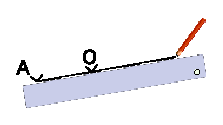
\includegraphics[width=3cm]{regleAO} &  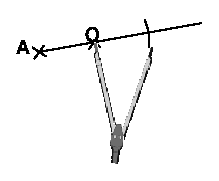
\includegraphics[width=3cm]{compasAO} & 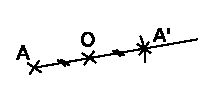
\includegraphics[width=3cm]{pointsAOA} \\ 
 On trace la demi-droite $[AO)$. & On trace un arc de cercle de centre $O$ et de rayon $OA$. Il coupe la demi-droite $[AO)$ en un point. & On place le point $A'$ à l'intersection de la demi-droite $[AO)$ et de l'arc de cercle. On code la figure. \\
\end{tabularx} \\
 \end{exemple*1}


\exercice
Trace un segment $[AB]$ de 5 cm de longueur puis construis le point $C$ symétrique de $B$ par rapport à $A$.
%\correction

\exercice
Trace un segment $[RT]$ de 8,4 cm de longueur, puis place le point $W$ tel que $R$ et $T$ soient symétriques par rapport au point $W$.
%\correction
 
\end{methode*1}

%%%%%%%%%%%%%%%%%%%%%%%%%%%%%%%%%%%%%%%%%%%%%%%%%%%%%%%%%%%%%%%%%%%%%

\begin{methode*1}[Construire le symétrique d'une figure]

\begin{aconnaitre}
\MotDefinition{Deux figures symétriques par rapport à un point}{} sont superposables après un demi-tour autour de ce point. 
\end{aconnaitre}

\begin{exemple*1}
Construis le symétrique de la figure $ABCD$ par rapport au point $O$ : \\[0.5em]
\begin{tabularx}{\textwidth}{X|X|X}
 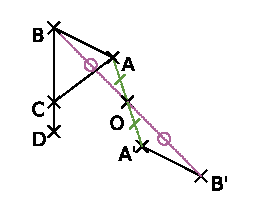
\includegraphics[width=3cm]{figure_sym1} &  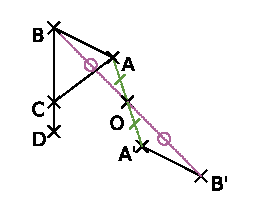
\includegraphics[width=3cm]{figure_sym2} & 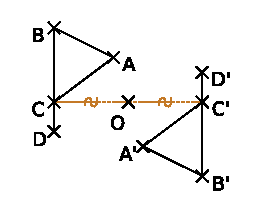
\includegraphics[width=3cm]{figure_sym3} \\ 
 On construit les points $A'$ et $B'$, symétriques des points $A$ et $B$ par rapport à $O$. On trace le segment $[A'B']$. & On construit  le point $D'$, symétrique du point $D$ par rapport à $O$. On trace le segment $[B'D']$. & On construit le point $C'$, symétrique du point $C$ par rapport à $O$. On trace le segment $[A'C']$. \\
\end{tabularx} \\
 \end{exemple*1}


\exercice
Trace un rectangle $ABCD$ tel que $AB = 4$ cm et $BC = 2,5$ cm. Trace le cercle de centre $B$ passant par $C$. Construis le symétrique de cette figure par rapport au point $D$.
%\correction
 
\end{methode*1}

%%%%%%%%%%%%%%%%%%%%%%%%%%%%%%%%%%%%%%%%%%%%%%%%%%%%%%%%%%%%%%%%%%%%%

\begin{methode*1}[Utiliser les propriétés de la symétrie centrale]

\begin{aconnaitre}
Si deux segments sont symétriques par rapport à un point alors \textbf{ils ont la même longueur}.

Si deux angles sont symétriques par rapport à un point alors \textbf{ils ont la même mesure}.

La symétrie centrale \textbf{conserve le périmètre et l'aire}.
\end{aconnaitre}

\begin{exemple*1}
Un triangle $PIC$ a un périmètre de 16,4 cm. Quel est le périmètre du triangle $PI'C'$ image de $PIC$ par la symétrie de centre $P$ ? Justifie ta réponse.\\[1em]
\correction
Les triangles $PIC$ et $PI'C'$ sont symétriques par rapport à un point : ils ont donc le même périmètre, c'est à dire 16,4 cm.
 \end{exemple*1}


\exercice
Les angles $\widehat{xOy}$ et $\widehat{x'Oy'}$, dont les mesures respectives sont $54^{\circ}$ et $55^{\circ}$, sont-ils symétriques par rapport au point $O$ ? Justifie ta réponse.
%\correction

\exercice
$ESV$ est un triangle rectangle en $E$. Quelle est la nature du triangle $E'S'V'$ image de $ESV$ par une symétrie centrale ? Justifie ta réponse.
%\correction
 
\end{methode*1}

